\documentclass[12pt]{article}
\usepackage{amsthm,amssymb,amsfonts,amsmath,amstext,systeme}
\usepackage{graphicx,float}
\usepackage{tabularx}

\marginparwidth 0pt
\oddsidemargin -1.2 truecm
\evensidemargin  0pt 
\marginparsep 0pt
\topmargin -2.2truecm
\linespread{1}
\textheight 25.8 truecm
\textwidth 18.5 truecm
\newenvironment{remark}{\noindent{\bf Remark }}{\vspace{0mm}}
\newenvironment{remarks}{\noindent{\bf Remarks }}{\vspace{0mm}}
\newenvironment{question}{\noindent{\bf Question }}{\vspace{0mm}}
\newenvironment{questions}{\noindent{\bf Questions }}{\vspace{0mm}}
\newenvironment{note}{\noindent{\bf Note }}{\vspace{0mm}}
\newenvironment{summary}{\noindent{\bf Summary }}{\vspace{0mm}}
\newenvironment{back}{\noindent{\bf Background}}{\vspace{0mm}}
\newenvironment{conclude}{\noindent{\bf Conclusion}}{\vspace{0mm}}
\newenvironment{concludes}{\noindent{\bf Conclusions}}{\vspace{0mm}}
\newenvironment{dill}{\noindent{\bf Description of Dill's model}}{\vspace{0mm}}
\newenvironment{maths}{\noindent{\bf Mathematics needed}}{\vspace{0mm}}
\newenvironment{inst}{\noindent{\bf Instructions}}{\vspace{0mm}}
\newenvironment{notes}{\noindent{\bf Notes }}{\vspace{0mm}}
\newenvironment{theorem}{\noindent{\bf Theorem }}{\vspace{0mm}}
\newenvironment{example}{\noindent{\bf Example }}{\vspace{0mm}}
\newenvironment{examples}{\noindent{\bf Examples }}{\vspace{0mm}}
\newenvironment{topics}{\noindent{\bf Topics}}{\vspace{0mm}}
\newenvironment{outcomes}{\noindent{\bf Expected Learning Outcomes}}{\vspace{0mm}}
\newenvironment{lemma}{\noindent{\bf Lemma }}{\vspace{0mm}}
\newenvironment{solution}{\noindent{\it Solution}}{\vspace{2mm}}
\newcommand{\ds}{\displaystyle}
\newcommand{\un}{\underline}
\newcommand{\bs}{\boldsymbol}

\begin{document}

\baselineskip 18 pt
\begin{center}
	{\large \bf HKDSE MATH CORE 2012 Past Paper I}\\
	\vspace{2 mm}

\end{center}
\vspace{0.05cm}

\begin{enumerate}
	\item \textbf{HKDSE MATH CORE 2012 Past Paper I Q1}\\
	Simplify $\dfrac{m^{-12}n^8}{n^3}$ and express your answer with positive indices. \\(3 marks)	
	
	\item \textbf{HKDSE MATH CORE 2012 Past Paper I Q2}\\
	Make $a$ the subject of the formula $\dfrac{3a+b}{8} = b-1$. \\(3 marks)

	\item \textbf{HKDSE MATH CORE 2012 Past Paper I Q3}\\
	Factorize
	\begin{enumerate}
		\item [(a)] $x^2 - 6xy + 9y^2$,
		\item [(b)] $x^2 - 6xy + 9y^2 + 7x - 21y$.
	\end{enumerate}
	(3 marks)

	\item \textbf{HKDSE MATH CORE 2012 Past Paper I Q4}\\
	The daily wage of Ada is 20\% higher than that of Billy while the daily wage of Billy is 20\% lower than that of Christine. It is given that the daily wage of Billy is \$480.
	\begin{enumerate}
		\item [(a)] Find the daily wage of Ada.
		\item [(b)] Who has the highest daily wage? Explain your answer.
	\end{enumerate}	
	(4 marks)
	
	\item \textbf{HKDSE MATH CORE 2012 Past Paper I Q5}\\
	There are 132 guards in an exhibition centre consisting of 6 zones. Each zone has the same number of guards. In each zone, there are 4 more female guards than male guards. Find the number of male guards in the exhibition centre. \\(4 marks)
	
	\item \textbf{HKDSE MATH CORE 2012 Past Paper I Q6}
	\begin{enumerate}
		\item [(a)] Find the range of values of $x$ which satisfy both $\dfrac{4x+6}{7} > 2(x-3)$ and $2x - 10\leq 0$.
		\item [(b)] How many positive integers satisfy both the inequalities in (a)?
	\end{enumerate}	
	(4 marks)

	\item \textbf{HKDSE MATH CORE 2012 Past Paper I Q7}\\
	The box-and-whisker diagram below shows the distribution of the times taken by a large group of students of an athletic club to finish a 100 m race:

	\begin{figure}[H]
		\centering
		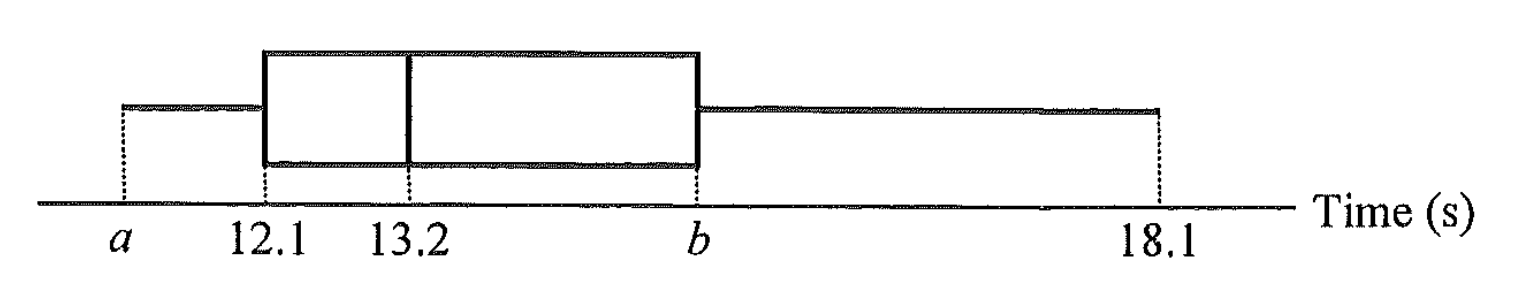
\includegraphics[width = .5\linewidth]{2012Figure1.0}
	\end{figure}

	The inter-quartile range and the range of the distribution are 3.2 s and 6.8 s respectively.

	\begin{enumerate}
		\item [(a)] Find $a$ and $b$.
		\item [(b)] The students join a training program. It is found that the longest time taken by the students to finish a 100 m race after the training is 2.9 s less than that before the training. The trainer claims that at least 25\% of the students show improvement in the time taken to finish a 100 m race after the training. Do you agree? Explain your answer.
	\end{enumerate}
	(4 marks)

	\item \textbf{HKDSE MATH CORE 2012 Past Paper I Q8}\\
	In Figure 1, $AB, BC, CD$ and $AD$ are chords of the circle. $AC$ and $BD$ intersect at $E$. It is given that $BE$ = 8 cm, $CE$ = 20 cm and $DE$ = 15 cm.
	\begin{figure}[H]
		\centering
		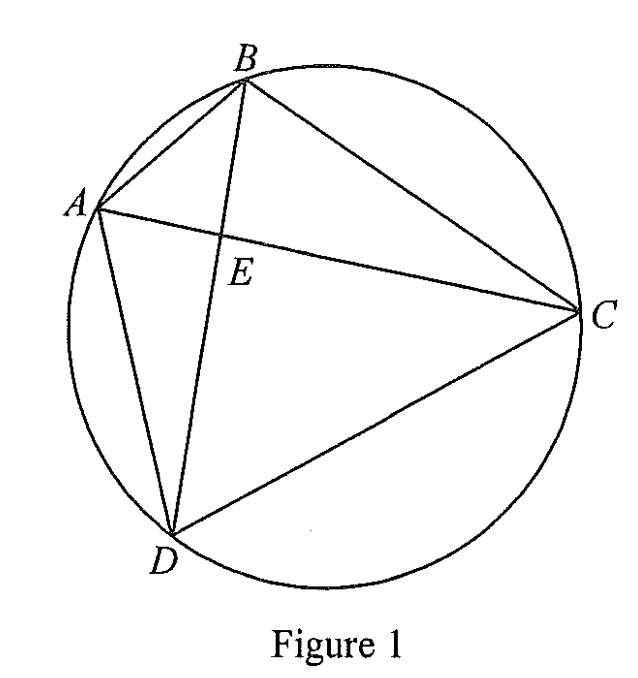
\includegraphics[width = .3
		\linewidth]{2012Figure1.1}
	\end{figure}
	\begin{enumerate}
		\item[(a)]Write down a pair of similar triangles in Figure 1. Also find $AE$.
		\item[(b)] Suppose that $AB$ = 10 cm. Are $AC$ and $BD$ perpendicular to each other? Explain your answer.
	\end{enumerate}
	(5 marks)


	\item \textbf{HKDSE MATH CORE 2012 Past Paper I Q9}\\
	In Figure 2, the volume of the solid right prism $ABCDEFGH$ is 1020 cm$^{3}$. The base $ABCD$ of the prism is a trapezium, where $AD$ is parallel to $BC$. It is given that $\angle BAD = 90^{\circ} $, $AB$ = 12 cm, $BC$ = 6 cm and $DE$ = 10 cm.
 
	\begin{figure}[H]
		\centering
		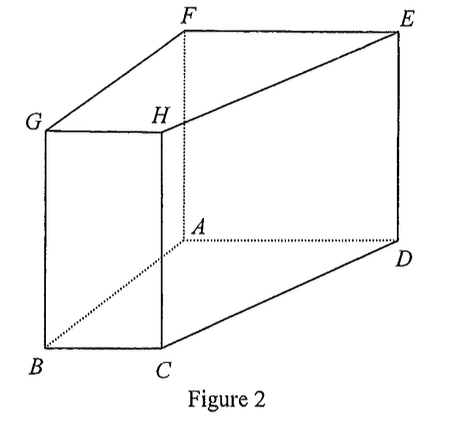
\includegraphics[width = .3\linewidth]{2012Figure1.2}
	\end{figure}
	Find
	\begin{enumerate}
		\item[(a)] the length of $AD$,
		\item[(b)] the total surface area of the prism $ABCDEFGH$.
	\end{enumerate}
	(5 marks)

	\item \textbf{HKDSE MATH CORE 2012 Past Paper I Q10}\\
	Tom conducts a survey on the numbers of hours spent on doing homework in a week by secondary students. Questionnaires are sent out and twenty of them are returned. The stem-and-leaf diagram below shows the numbers of hours recorded in the twenty questionnaires:
	\begin{table}[htbp]
		\centering
		\begin{tabular}{r|l@{\hspace{4 pt}}l@{\hspace{4 pt}}l@{\hspace{4 pt}}}
		   Stem (tens) & Leaf (units)     \\
			\hline
			1     & 0 0 1 1 2 3 4 5 5 6 6 7 7\\    
			2     & 0 0 0 5 8\\    
			3     & 4 6\\    
		\end{tabular}
		\label{tab:addlabel}
	\end{table}
	\begin{enumerate}
		\item[(a)] Find the mean and the median of the numbers of hours recorded in the twenty questionnaires. \\(2 marks)
		\item[(b)] Tom receives four more questionnaires. He finds that the mean of the numbers of hours recorded these four questionnaires is 18. It is found that the numbers of hours recorded in two of these four questionnaires are 19 and 20.
		\begin{enumerate}
			\item [(i)]	Write down the mean of the numbers of hours recorded in the twenty-four questionnaires.
			\item [(ii)] Is it possible that the median of the numbers of hours recorded in the twenty-four questionnaires is the same as the median found in (a)? Explain your answer.	
		\end{enumerate}		
		(4 marks)
	\end{enumerate}

	
	\item \textbf{HKDSE MATH CORE 2012 Past Paper I Q11}\\
	Let \$ $C$ be the cost of painting a can of surface area $A$ m$^2$. It is given that $C$ is the sum of two parts, one part is a constant and the other part varies as $A$. When $A$ = 2, $C$ = 62; when $A$ = 6, $C$ = 74.
	\begin{enumerate}
		\item[(a)] Find the cost of painting a can of surface area 13 m$^2$. \\(4 marks)
		\item[(b)] There is a larger can which is similar to the can described in (a). If the volume of the larger can is 8 times that of the can described in (a), find the cost of painting the larger can. \\ (2 marks)
	\end{enumerate}


	\item \textbf{HKDSE MATH CORE 2012 Past Paper I Q12}\\
	Figure 3(a) shows a solid metal right circular cone of base radius 48 cm and height 96 cm.
 
	\begin{figure}[H]
		\centering
		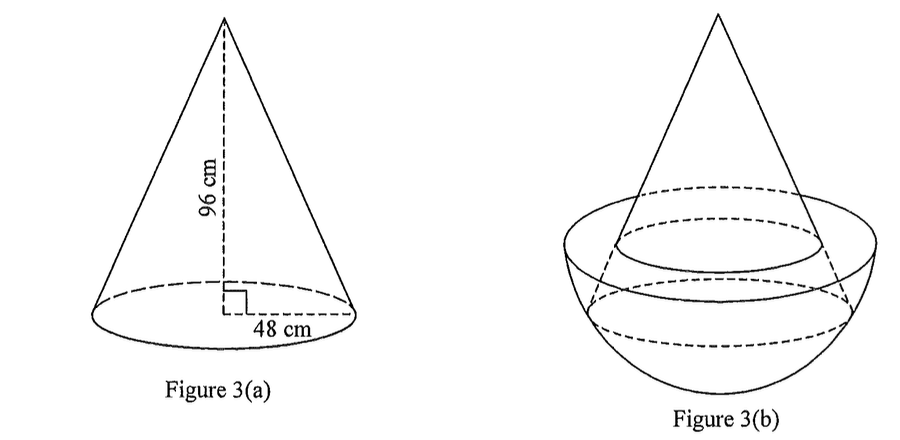
\includegraphics[width = .3\linewidth]{2012Figure1.3}
	\end{figure}
	\begin{enumerate}
		\item[(a)] Find the volume of the circular cone in terms of $\pi$.\\(2 marks)
		\item[(b)] A hemispherical vessel of radius 60 cm is held vertically on a horizontal surface. The vessel is fully filled with milk.
		\begin{enumerate}
			\item[(i)] Find the volume of the milk in the vessel in terms of $\pi$.
			\item[(ii)] The circular cone is now held vertically in the vessel as shown in Figure 3(b). A craftman claims that the volume of the milk remaining in the vessel is greater than 0.3 m$^3$. Do you agree? Explain your answer. 
		\end{enumerate}
		(5 marks)
	\end{enumerate}

	\item \textbf{HKDSE MATH CORE 2012 Past Paper I Q13}
	\begin{enumerate}
		\item[(a)] Find the value of $k$ such that $x - 2$ is a factor of $kx^3 - 21x^2 + 24x - 4$. \\(2 marks)
		\item[(b)] Figure 4 shows the graph of $y = 15x^2 - 63x + 72$. $Q$ is a variable point on the graph in the first quadrant. $P$ and $R$ are the feet of the perpendiculars from $Q$ to the $x$-axis and the $y$-axis respectively.
		\begin{figure}[H]
			\centering
			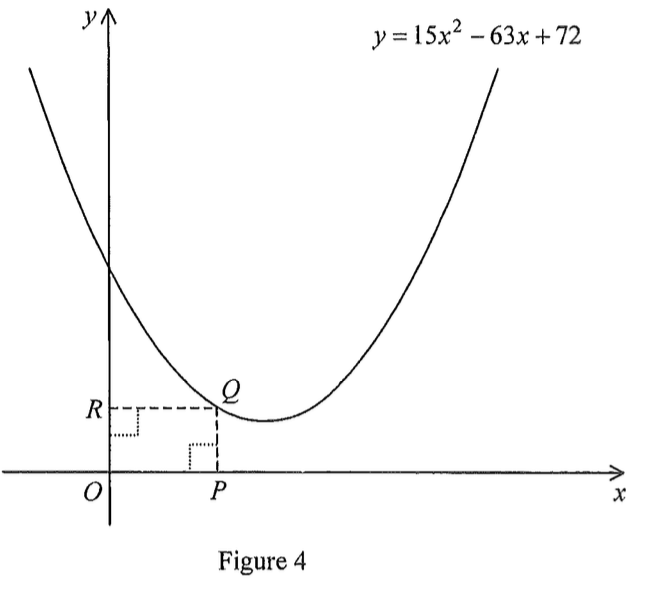
\includegraphics[width = .3\linewidth]{2012Figure1.4}
		\end{figure}
		\begin{enumerate}
			\item[(i)] Let $(m, 0)$ be the coordinates of $P$. Express the area of the rectangle $OPQR$ in terms of $m$.
			\item[(ii)] Are there three different positions of $Q$ such that the area of the rectangle $OPQR$ is 12? Explain your answer.
		\end{enumerate}
		(5 marks)
	\end{enumerate}

	\item \textbf{HKDSE MATH CORE 2012 Past Paper I Q14}\\
	The $y$-intercepts of two parallel lines $L$ and $l$ are $-1$ and $-3$ respectively and the $x$-intercept of $L$ is 3. $P$ is a moving point in the rectangular coordinate plane such that the perpendicular distance from $P$ to $L$ is equal to the perpendicular distance from $P$ to $l$. Denote the locus of $P$ by $\Gamma$.
	\begin{enumerate}
		\item[(a)]\begin{enumerate}
			\item[(i)] Describe the geometric relationship between $\Gamma$ and $L$.
			\item[(ii)] Find the equation of $\Gamma$.
		\end{enumerate}
		(5 marks)
		\item[(b)] The equation of the circle C is $(x-6)^2 + y^2 = 4$. Denote the centre of $C$ by $Q$.
		\begin{enumerate}
			\item[(i)] Does $\Gamma$ pass through $Q$? Explain your answer.
			\item[(ii)] If $L$ cuts $C$ at $A$ and $B$ while $\Gamma$ cuts $C$ at $H$ and $K$, find the ratio of the area of $\triangle AQH$ to the area of $\triangle BQK$.
		\end{enumerate}
		(4 marks)
	\end{enumerate}

	\item \textbf{HKDSE MATH CORE 2012 Past Paper I Q15}\\
	The standard deviation of the test scores obtained by a class of students in a Mathematics test is 10 marks. All the students fail in the test, so the test score of each student is adjusted such that each score is increased by 20\% and then extra 5 marks are added.
	\begin{enumerate}
		\item[(a)] Find the standard deviation of the test scores after the score adjustment. \\(1 mark)
		\item[(b)] Is there any change in the standard score of each student due to the score adjustment? Explain your answer. \\(2 marks)
	\end{enumerate}
	
	\item \textbf{HKDSE MATH CORE 2012 Past Paper I Q16}\\
	There are 8 departments in a company. To form a task group of 16 members, 2 representatives are nominated by each department. From the task group, 4 members are randomly selected.
	\begin{enumerate}
		\item[(a)] Find the probability that the 4 selected members are nominated by 4 different departments. \\(2 marks)
		\item[(b)] Find the probability that the 4 selected members are nominated by at most 3 different departments. \\(2 marks)
	\end{enumerate}

	\item \textbf{HKDSE MATH CORE 2012 Past Paper I Q17}\\
	The coordinates of the centre of the circle $C$ are $(6, 10)$. It is given that the $x$-axis is a tangent to $C$.
	\begin{enumerate}
		\item[(a)] Find the equation of $C$. \\(2 marks)
		\item[(b)]The slope and the $y$-intercept of the straight line $L$ is $-1$ and $k$ respectively. If $L$ cuts $C$ at $A$ and $B$, express the coordinates of the mid-point of $AB$ in terms of $k$. \\(5 marks)
	\end{enumerate}

	\item \textbf{HKDSE MATH CORE 2012 Past Paper I Q18}\\
	Figure 5(a) shows a right pyramid $VABCD$ with a square base, where $\angle VAB = 72^\circ$. The length of a side of the base is 20 cm. Let $P$ and $Q$ be the points lying on $VA$ and $VD$ respectively such that $PQ$ is parallel to $BC$ and $\angle PBA = 60^\circ$. A geometric model is made by cutting off the pyramid $VPBCQ$ from $VABCD$ as shown in Figure 5(b).
	\begin{figure}[H]
		\centering
		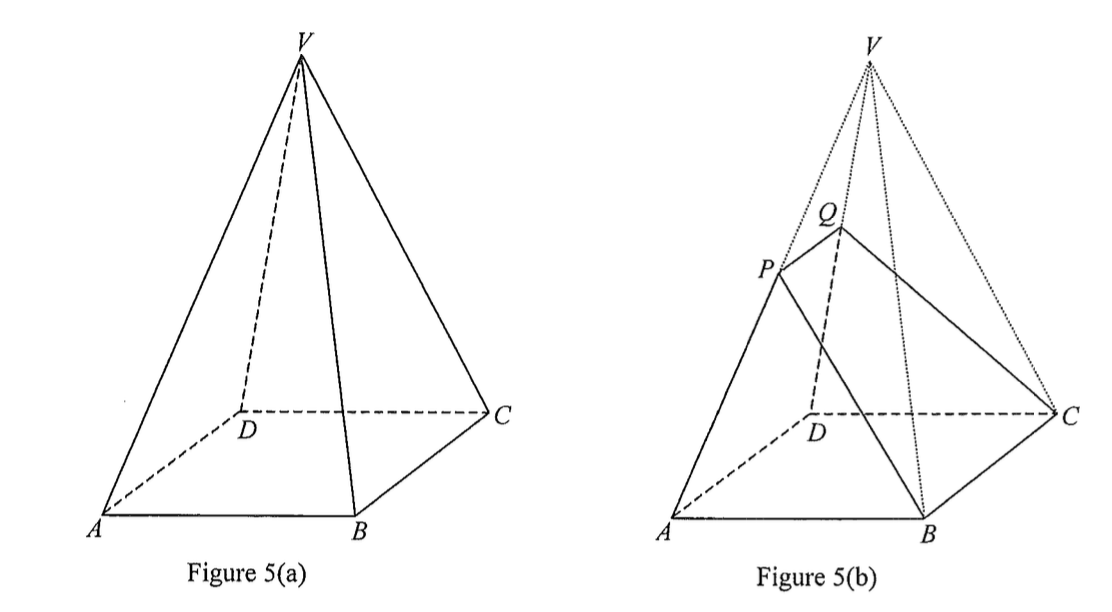
\includegraphics[width = .3\linewidth]{2012Figure1.5}
	\end{figure}
	\begin{enumerate}
		\item[(a)] Find the length of AP. \\(2 marks)
		\item[(b)] Let $\alpha$ be the angle between the plane $PBCQ$ and the base $ABCD$.	
		\begin{enumerate}
			\item[(i)] Find $\alpha$.
			\item[(ii)] Let $\beta$ be the angle between $PB$ and the base $ABCD$. Which one of $\alpha$ and $\beta$ is greater? Explain your answer.	
		\end{enumerate}
		(6 marks)
	\end{enumerate}

	\item \textbf{HKDSE MATH CORE 2012 Past Paper I Q19}\\
	In a city, the air cargo terminal $X$ of an airport handles goods of weight $A(n)$ tonnes in the $n$th year since the start of its operation, where $n$ is a positive integer. It is given that $A(n) = ab^{2n}$, where $a$ and $b$ are positive constants. It is found that the weights of the goods handled by $X$ in the 1st year and the 2nd year since the start of its operation are 254 100 tonnes and 307 461 tonnes respectively.

	\begin{enumerate}
		\item[(a)]
		\begin{enumerate}
			\item[(i)] Find $a$ and $b$. \\
			Hence find the weight of the goods handled by $X$ in the 4th year since the start of its operation.
			\item[(ii)] Express, in terms of $n$, the total weight of the goods handled by $X$ in the first $n$ years since the start of its operation.
		\end{enumerate}
		(6 marks)
		\item[(b)] The air cargo terminal $Y$ starts to operate since $X$ has been operated for 4 years. Let $B(m)$ tonnes be the weight of the goods handled by $Y$ in the $m$th year since the start of its operation, where $m$ is a positive integer. It is given that $B(m) = 2ab^m$.
		\begin{enumerate}
			\item[(i)] The manager of the airport claims that after $Y$ has been operated, the weight of the goods handled by $Y$ is less than that handled by $X$ in each year. Do you agree? Explain your answer.
			\item[(ii)] The supervisor of the airport thinks that when the total weight of the goods hangled by $X$ and $Y$ since the start of the operation of $X$ exceeds 20 000 000 tonnes, new facilities should be installed to maintain the efficiency of the air cargo terminals. According to the supervisor, in which year since the start of the operation of $X$ should the new facilities be installed?
		\end{enumerate}
		(7 marks)
	\end{enumerate}
\end{enumerate}


\end{document}